\documentclass[11pt]{article}
\usepackage[utf8]{inputenc}
\usepackage{amsmath,amssymb,hyperref,array,xcolor,multicol,verbatim,mathpazo}
\usepackage[normalem]{ulem}
\usepackage[pdftex]{graphicx}
\usepackage{fullpage}
\usepackage{import}
\usepackage{adjustbox}
\usepackage{booktabs}
\usepackage[font=footnotesize,labelfont=bf]{caption}
\captionsetup{justification=raggedright,singlelinecheck=false}


\usepackage[backend=biber,style=authoryear,
sorting=ynt,citestyle=authoryear]{biblatex}
\addbibresource{papercitations.bib}
\usepackage{setspace}
\singlespacing
\addtolength{\skip\footins}{2pc plus 5pt}

\title{Labor Markets and Technological Change: Evidence from Electronic Health Records}
\author{Hanna Glenn}
%\date{\today}

\DeclareLabeldate[online]{%
  \field{date}
  \field{year}
  \field{eventdate}
  \field{origdate}
  \field{urldate}
}

\begin{document}

\maketitle



\vspace{1.5cm}

The relationship between technological innovation and labor markets is a longstanding topic of interest in economics and in policy making. Their interaction has direct impacts across industries; job changes such as displacement, creation, and satisfaction are all prevalent for many workers (\cite{autor2003skill}, \cite{fallick1996review}, \cite{akerlof1988job}). Labor market changes for one job type may also have rippling effects on populations serviced by that industry. One such job is that of a physician, where physician choices and labor markets directly affect patients on margins of accessibility and quality of care received. For example, physician burnout is correlated with lower patient satisfaction (\cite{shanafelt2002burnout}), physician shortages are linked to higher mortality rates (\cite{gong2019higher}), and administrative regulations such as standardized checklists may be associated with lower mortality in surgical settings (\cite{treadwell2014surgical}). Thus, shocks to physician labor markets or work settings may have drastic implications for patients. I investigate physician labor markets under a major technology change in the U.S. healthcare system, the implementation of electronic health care record systems, which have been emphasized as a cause of burnout and may induce changes to physician labor market decisions.

Electronic Health Records (EHRs) are computerized medical records which include detailed accounts and notes of medical history, stored in advanced systems with additional capabilities such as providing suggesions for care. EHRs have have become increasingly relevant in the U.S. since 2008, in part after former President Obama stated in 2009, “To improve the quality of our health care while lowering its cost, we will make the immediate investments necessary to ensure that, within five years, all of America’s medical records are computerized.” (\cite{presquote}). The movement towards digitization in health care was expected to have immediate and substantial impacts on efficiency. A 2005 study estimated hundreds of billions of dollars saved if health information technology were to be fully implemented (\cite{hillestad2005}). Such expectations led the U.S. government to incentivize the use of EHRs in hospitals with the the Health Information Technology for Economic and Clinical Health (HITECH) Act in 2008 (\cite{hitech})\footnote{This legislation subsidized hospitals which used EHRs “meaningfully”According to Quatris Healthco, meaningful use standards proceeded in three stages over time. In Stage 1 (2010), MU focused on data capturing and sharing. In Stage 2, which began in late 2012, MU extended to using EHRs for patient incorporation and using the technology as a helper in care. Stage 3 went from 2014-2016 and focused on making data accessible across hospitals (\cite{meanuse})}. The percentage of hospitals with the capability of using a basic EHR system went from 9 percent in 2008 to 84 percent in 2015 (\cite{stats}), evidence of the nationwide movement towards digitization.

Physicians, as primary users of this technology, have a meaningful role in whether potential benefits of EHRs are realized. However, with the rapid implementation of EHRs, the day to day life of physicians also changed rapidly. In interviews, physicians reported that when using EHRs they are less satisfied with their job and have higher stress levels. Senior physicians in particular were found to “loathe the cumbersome, time-consuming data entry that comes with using EHRs.” (\cite{CollierBurnout}). The frustration of using a new technology raises the cost of working in specific hospitals, which may lead physicians on the margin to make changes in labor market choices such as exiting the labor force altogether. Further, the short and long run impacts of EHRs on physician productivity could vary greatly due to the immediate learning curve that subsides over time.  I use difference in difference with heterogeneous treatment timing to understand the effect of EHR implementation in hospitals on physician labor market outcomes: retirement, choice of work setting, and patients seen in the short vs. long run.

Using CMS Shared Patient data and Medicare Data on Provider Practice and Specialty (MD-PPAS), I construct a physician-level panel on hospitalists and other general practice physicians connected to hospitals from 2009-2017. The data captures the extent to which the physician in exposed to EHRs in hospitals, various labor market outcomes, and demographic information such as zip code, age, and gender. I analyze the impact of EHR exposure on the following physician decisions: (1) retirement, (2) where to physically work (changing hospitals or moving to office based settings), and (3) the number of patients seen by the physician. Common to each specification is the use of treatment variables capturing a physicians' level of EHR exposure in hospitals. I consider exposure on two dimensions: working in any hospital that implements an EHR, and working in a low-integrated hospital that implements an EHR.  To study retirement, I focus primarily on the sample of older physicians who are closer to the margin of retirement, since the opportunity cost of retiring for a young physician is very high and the cost of using an EHR is unlikely to exceed it. Contrary to previous work stating that physicians do not retire based on work environment (\cite{Bahrami2002}), I find that \textcolor{red}{put exact findings here. (The funny thing is, I find that young physicians "retire"... I need to figure out what this means and possibly rephrase the last couple sentences)}.

For those who stay in the labor force, there may be margin to change physicil place of work if physicians are unhappy with the specific loss of autonomy experienced at a given hospital. That is, do physicians switch from primarily hospital based work to smaller office based settings, or do they switch hospital locations where the technology looks different? To answer this question, I limit the sample to any physicians who stay in the labor force after EHR exposure and use the same event study framework to estimate the effect on whether the physician switches zip codes or increases office-based patients. I find that \textcolor{red}{put exact findings here and their implications (are physicians trying to shift away from an autonomous standard of care they have to abide by?)}. 

Finally, I investigate the effect of the technology implementation on productivity within hospitals, measured by the number of patients seen. The population of physicians left in this analysis are those who do not retire or switch to an office based setting. I find that the number of patients seen does not change in the immediate years after implementation, and that it takes two years after exposure to see productivity gains. After 5 years of exposure, a physician is seeing on average 11\% more patients relative to before EHRs. This result speaks to the disconnect between expected effects and realized effects of EHRs which is discussed in the health information technology literature. Since more patients are being seen by physicians, efficiency and access to care have both increased while costs (Medicaid patients) and quality remain unchanged. \textcolor{red}{This paragraph needs some work as my results have changed since getting the MDPPAS data and I need to push on other mechanisms besides productivity - if other physicians left and work had to be picked up or billing activity increased or demand increased (maybe due to ACA?)}

A key assumption underlying this analysis is that EHR exposure is exogenous to individual physicians. That is, a hospital makes the decision to implement an EHR independent of a physicians' labor market response to that implementation. This assumption is not unrealistic in large hospitals who employ many physicians, but may be violated in small hospitals where a physician has a voice in management. To address this, I first limit the analysis to large hospitals. However, small hospitals are especially important in studying patient access to care. To include small hospitals in the analysis, I instrument EHR adoption with local bandwidth capacity. \textcolor{red}{Relate these findings to previous findings. I need to make this paragraph more clear as I improve what I'm doing}

\textcolor{red}{Add a paragraph discussing sensitivity analysis or mechanisms.}

This paper's contribution to the space is threefold: (1) this is the first study to my knowledge that empirically analyzes the relationship between physician labor markets and EHRs, (2) since there seems to be a disconnect between the potentials of EHR technologies and the realized effects, this paper will speak to a potential mechanism that is causing this puzzle, and (3) this study covers the time period of the major EHR boom in healthcare, whereas most studies mentioned above utilize data before 2010. \textcolor{red}{This needs to be expounded upon a lot. Perhaps one or two paragraphs for each area of contribution.}

The effects of EHR implementation on costs and quality of healthcare prior to 2010 have been studied extensively. Despite many case studies and hospital-level analysis that indicate a large decrease in mortality rates (\cite{Buntin2011TheResults}), more recent economic research has showed that the technology has only improved health outcomes for patients with severe conditions, but have not led to improvements for the median patient (\cite{Agha2014TheCare}; \cite{McCullough2016HealthCoordination}; \cite{Meyerhoefer}). Further, there have been no significant cost decreases due to EHRs in the short or long run. If any cost reductions are realized at all, they are at least 6 years after implementation (\cite{dranove2014trillion}). As discussed earlier, these findings are puzzling due to the expected benefits of EHRs. This paper contributes to our knowledge of this area in re-framing past finding into a patient access to care problem instead of an efficiency problem.

\textcolor{red}{Expand both contribution and literature review and combine them to flow better.}


\newpage


\section{Background}

EHRs have been an important feature of healthcare since the 1980s and 1990s. Early in its existence, the technology was mainly produced and used by academic medical centers whose primary goal was to create efficiency in billing and scheduling. Before the rapid development of computers, physicians were not even able to interface directly with EHRs, and thus were not drastically affected. The cost of utilizing an EHR was extremely large, and cost increased as the amount of capabilities increased, which led to the widespread view that EHRs were strictly complements to paper records and not a feasible substitute. The possibility of using solely EHRs increased as computers became more portable, creating what is known as the "physician workspace": a computer station for a physician to interface directly with EHRs to record patient updates. However, physicians kept the view that EHRs were purely complementary to paper due to burdensome data entry. Automation in data entry was non-existent, making it extremely time consuming for the user. Even when automation was developed for particular machines that performed monitoring, the hospital still held responsible for the accuracy of information and therefore required physicians to double check each data entry. 

The HITECH Act was passed in 2009, setting aside government funds to subsidize hospitals who used EHRs according to certain guidelines. These requirements include having at least 80\% of patients in the system, recording answers to specific questions, and protecting the security of the system to ensure privacy. Immediately, EHR companies took advantage of the legislation and began marketing campaigns centered around their system being eligible to earn the hospital subsidies. Hospitals began receiving payments for the first stage of meaningful use in 2011. This led to a 75 percentage point increase in the number of hospitals with EHRs from 2009 to 2015 (\cite{stats}). \textcolor{red}{maybe put HealthIT US map that shows hospitals who received incentive payment?} While EHRs are widely implemented in hospitals by 2015, physicians still continue to report frustration. "Some healthcare professionals continue to develop workarounds and rely on paper alternatives rather than using EHRs" (\cite{evans2016electronic}).  

\section{Data}

Using various linked datasets, I construct a physician-level panel spanning from 2009-2017 which measures physicians' exposure to EHRs over time and other relevant characteristics. The different data sets used to construct this panel are described below.

\subsection{MD-PPAS}

Medicare Data on Provider Practice and Specialty is a database of physicians designed to record information about claim counts and specialty from 2009-2017. The relevant information included is physician NPI, primary and secondary specialties, patient counts in up to 12 different zip codes, and fraction of patients in different settings such as office, inpatient or emergency room. First, I make limitations to the sample of physicians based on specialty type. Primary care physicians are the most likely to be exposed to the administrative burden of EHRs in hospitals. Thus, I only include physicians whose primary specialty is hospitalist, internal medicine, pediatrics, general practice or family practice in at least one year (excluding physicians who have specialist listed for all other years). Since the focus of the analysis is physicians working in hospitals, I also drop physicians with less than 20\% of patients in a hospital setting in all years. 
The dependent variables are constructed using MD-PPAS claim and patient count information. Retirement is an indicator variable that is equal to 1 in the first year that all future claims in all zip codes are equal to 0. I do not observe retirement in 2017, and drop those who "retire" in 2016 since one year of zero claims does not necessarily mean retirement.  

\subsection{Shared Patient}

CMS Shared Patient data records the number of patients who bill two entities under Medicaid in the same day. For example, if a Medicaid patient is referred to a specialist by a primary care physician, then those two physicians have a shared patient in common. I limit the entities by NPI tax-code to only include shared patients for physician-hospital pairs. I care specifically about physicians who have a close working relationship with hospitals, preferably those who do rounds within at least one hospital. To achieve this, I limit the qualifications for a sufficient physician-hospital pair. First, I only consider doctors who have a primary care role, excluding any specialists. The reason for this is that a primary care physician who does rounds in a hospital is likely to be primarily employed by that hospital (not brought in from a practice). Another reason for this is that primary care doctors interact directly with EHRs during checkups, unlike a surgeon. Second, I limit pairs to those which have a substantial number of patients billed together in the same day. This is to avoid including the potential physician who works in an office but happens to send a small number of patients to a nearby hospital. I consider a substantial number of patients to be at least 30 patients bill both the physician and the hospital in the same day in at least one year, \textcolor{red}{where the exact number chosen is explored in the appendix}. The physicians remaining in the data are likely doing a number of rounds physically inside hospitals, since it is unlikely that many patients will see a primary care doctor in a private office and then immediately go to a hospital in the same day. 

Using hospital NPI, I link the physician-hospital pairs to the American Hospital Association survey, which contains information on hospital-level EHR use and other characteristics. I then aggregate to the physician level, where physician EHR use is measured as the percentage of their hospitals which use an EHR in a given year. Additional physician-level characteristics, such as years of experience, come from Physician Compare. 

Overall summary statistics of the variables are shown in \hyperref[fig:summarystatistics]{Table 1}. Average hospital operating days is a physician-level variable that averages the number of operating days for that physicians hospital network. While there are some low outliers with a low value, on average physicians are working in hospitals open year round. Similarly, the average size of the hospital worked with averages the number of beds of each hospital in a physician's network. While these two average variables can technically vary by year, they tend to stay constant across the data, which is why they are included in the static category. Approximately 30\% of the sample of physicians are female and the average physician graduated medical school in 1993. Note that there are no physicians in the data who graduated after 2009, since they would be entering the labor force during the span of the data. On average, a physician works with between 1 and 2 hospitals as well as hospital systems. While the number of hospitals that a physician cares for patients in varies by year, the number of hospitals in their network is constant. The physician level variables that vary over time deal are the treatment variables regarding EHR exposure and the number of Medicaid patients seen. For all physician-years, physicians were exposed to an EHR in 56\% of the hospitals they work in and 70\% of the sample is exposed to any EHR. Once a physician becomes exposed to an EHR, they cannot go back to being unexposed. Finally, physicians are seeing an average of 620 Medicaid patients in hospitals per year.

\vspace{5mm}
\begin{table}[ht]
    \import{Table Code}{overall stats.tex}
    \label{fig:summarystatistics}
    \vspace{1mm}
    \caption*{\footnotesize Obs: 1,044,001}
\end{table}
\vspace{5mm}

I also include summary statistics by year and physician experience for comparison in Table \textcolor{red}{number}. In all years, senior physicians see more patients on average than younger physicians. Note that in 2015 the number of Medicaid patients drops drastically. This is due to the data collection in 2015 cutting off earlier than previous years since it was the last year collected for the data set. Because of this limitation, I drop 2015 in the productivity analysis, where number of patients is the dependent variable. 

\textcolor{red}{I need to think about why senior physicians are more exposed than younger physicians}



\vspace{5mm}
\begin{table}[ht]
\caption{Summary Statistics by Year and Experience Level}
\import{Table Code}{split stats.tex}
\end{table}
\vspace{5mm}




For a clear look at the variation in treatment variables over time, \hyperref[fig:figure1]{Figure 1} shows the average of these variables over time. In 2009, 42\% of the sample of physicians were exposed to an EHR. That is, over half of the sample had no affiliation with EHRs at the beginning of the sample period. By 2015, 92\% of physicians had exposure to an EHR in at least one hospital in their network. Similarly, the fraction of hospitals in a physician's network which were using an EHR was 30\% in 2009 and grew to 82\% in 2015. These statistics are consistent with the surge in incentives to implement EHRs in hospitals. 

\vspace{5mm}
\begin{figure}[ht]
    \caption{Treatment Variables Over Time}
    \vspace{-2mm}
    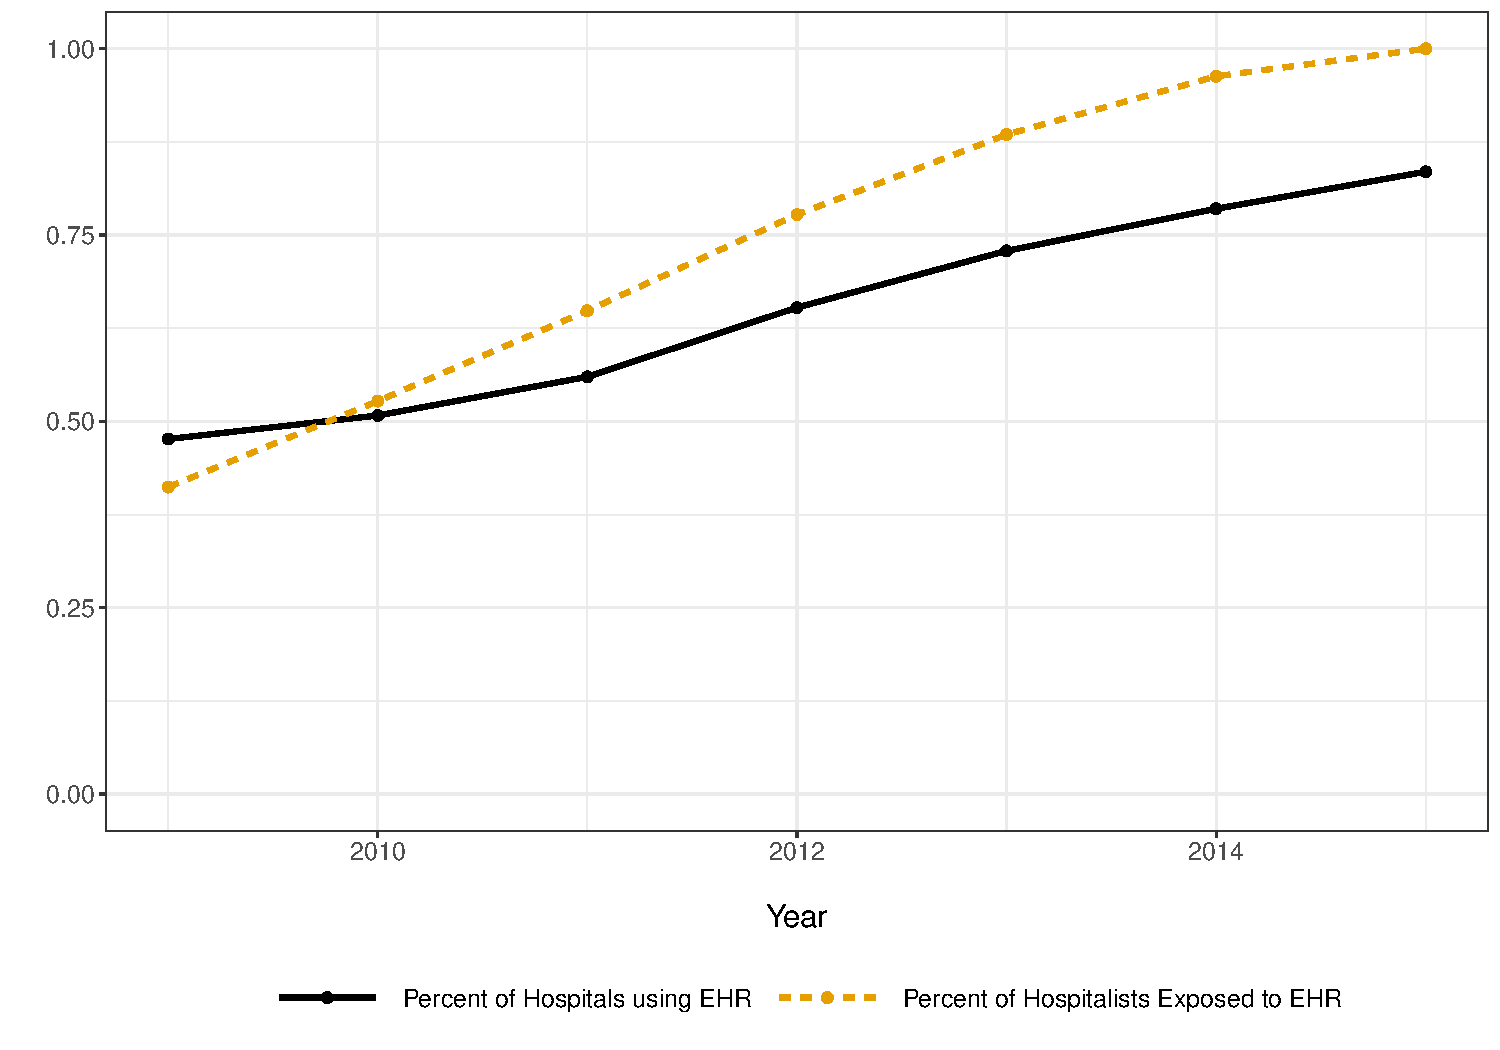
\includegraphics[scale=.5]{Objects/sum_stats_year.pdf}
    \label{fig:figure1}
\end{figure}
\vspace{5mm}

\newpage

\section{Retirement}

It is not uncommon in developed countries for workers to plan for retirement well in advance. Many workers have a retirement age set and spend their working life saving to get to that point. An exogenous shock typically will not change this retirement age because of the large sum of money necessary to formally leave the labor force. However, physicians typically make this decision differently than the majority of workers. Most physicians plan to retire at age 60, but do not actually retire until age 69 (\cite{collier2017challenges}). The reason being that the type of person who selects into being a physician will, on average, have a high regard for helping people. When it comes time to retire, they hesitate to abandon patients they have seen over the course of their career. This decision to delay retirement is not financial. Thus, retiring may be in a physician's choice set years before the realized decision to leave the labor force. 

This implies that an exogenous shock to work setting could, if it outweighs the concern for patients, cause an earlier exit. Medical articles suggest that the implementation of EHRs did lead to retirement in older physicians. \textcolor{red}{cite articles}. 

\subsection{Event Study and Results}

Figure \ref{fig:retirefirst} shows the aggregated group time treatment effects of being exposed to an EHR in a hospital. The left panel of the figure includes all physicians and shows a clear increase in the probability of retiring after exposure to an EHR. On the right panel, only physicians over the age of 50 are included. These results are puzzling, as they show that young physicians are the ones "retiring", or leaving the labor force. \textcolor{red}{However, this may just reflect that in later years taking a one or two year break looks like retiring whereas in early years it doesn't. What would cause a physician to drop out of the data for one or two years? Add to the appendix the same analysis but dropping physicians who "retired" after 2014. }

\begin{figure}[ht]
\caption{}
        \begin{minipage}[b]{0.47\linewidth}
            \centering
            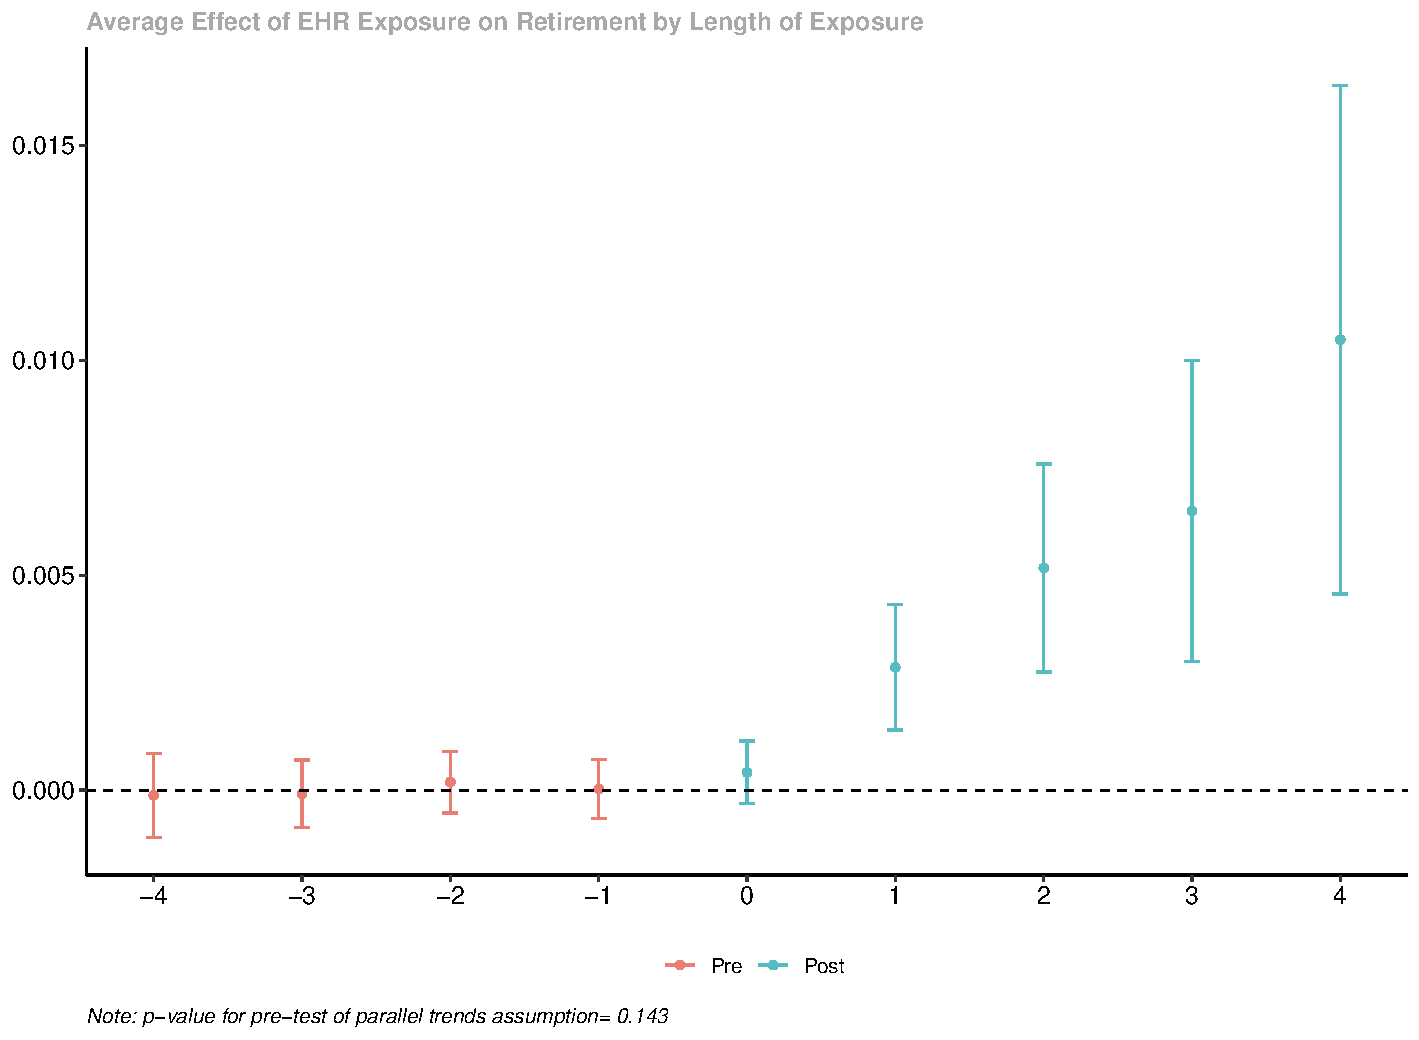
\includegraphics[width=\textwidth]{Objects/ggdid_retire_allEHR.pdf}
        \end{minipage}
        \hspace{0.2cm}
        \begin{minipage}[b]{0.47\linewidth}
            \centering
            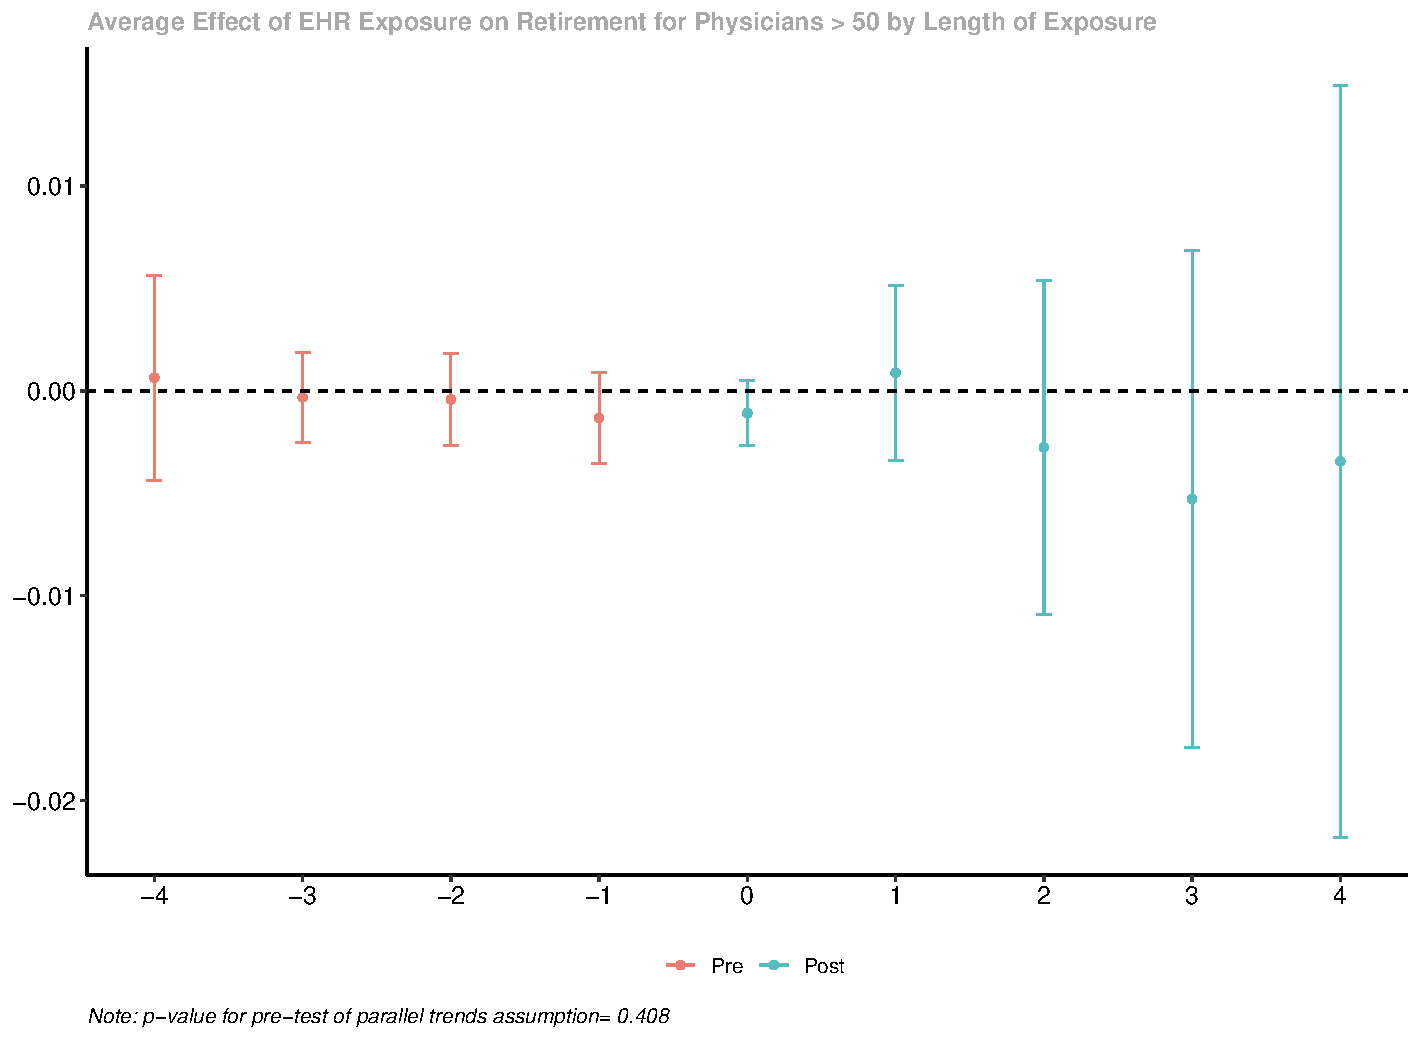
\includegraphics[width=\textwidth]{Objects/ggdid_retire_allEHR_old.pdf}
        \end{minipage}
        \label{fig:retirefirst}
\end{figure}

I also repeat this analysis with a more strict version of exposure to EHRs. A physician is only considered exposed if they worked in a low-integration status hospital that implemented an EHR. These results are shown in Figure \ref{fig:retiresecond}. 

\begin{figure}[ht]
\caption{}
        \begin{minipage}[b]{0.47\linewidth}
            \centering
            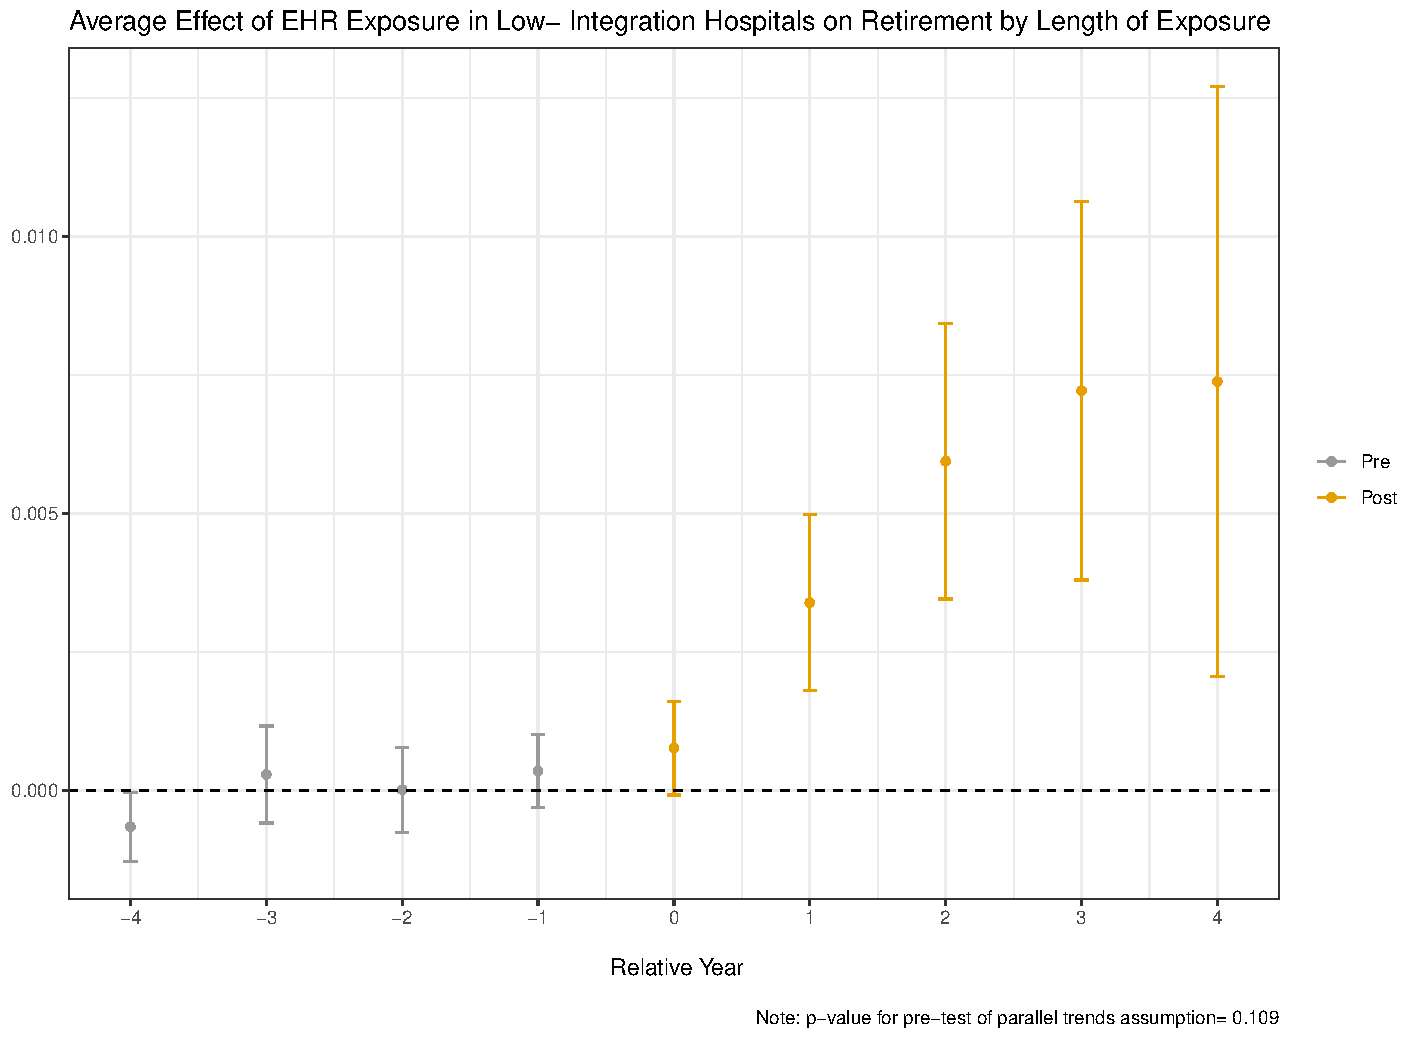
\includegraphics[width=\textwidth]{Objects/ggdid_retire_allEHR_li.pdf}
        \end{minipage}
        \hspace{0.2cm}
        \begin{minipage}[b]{0.47\linewidth}
            \centering
            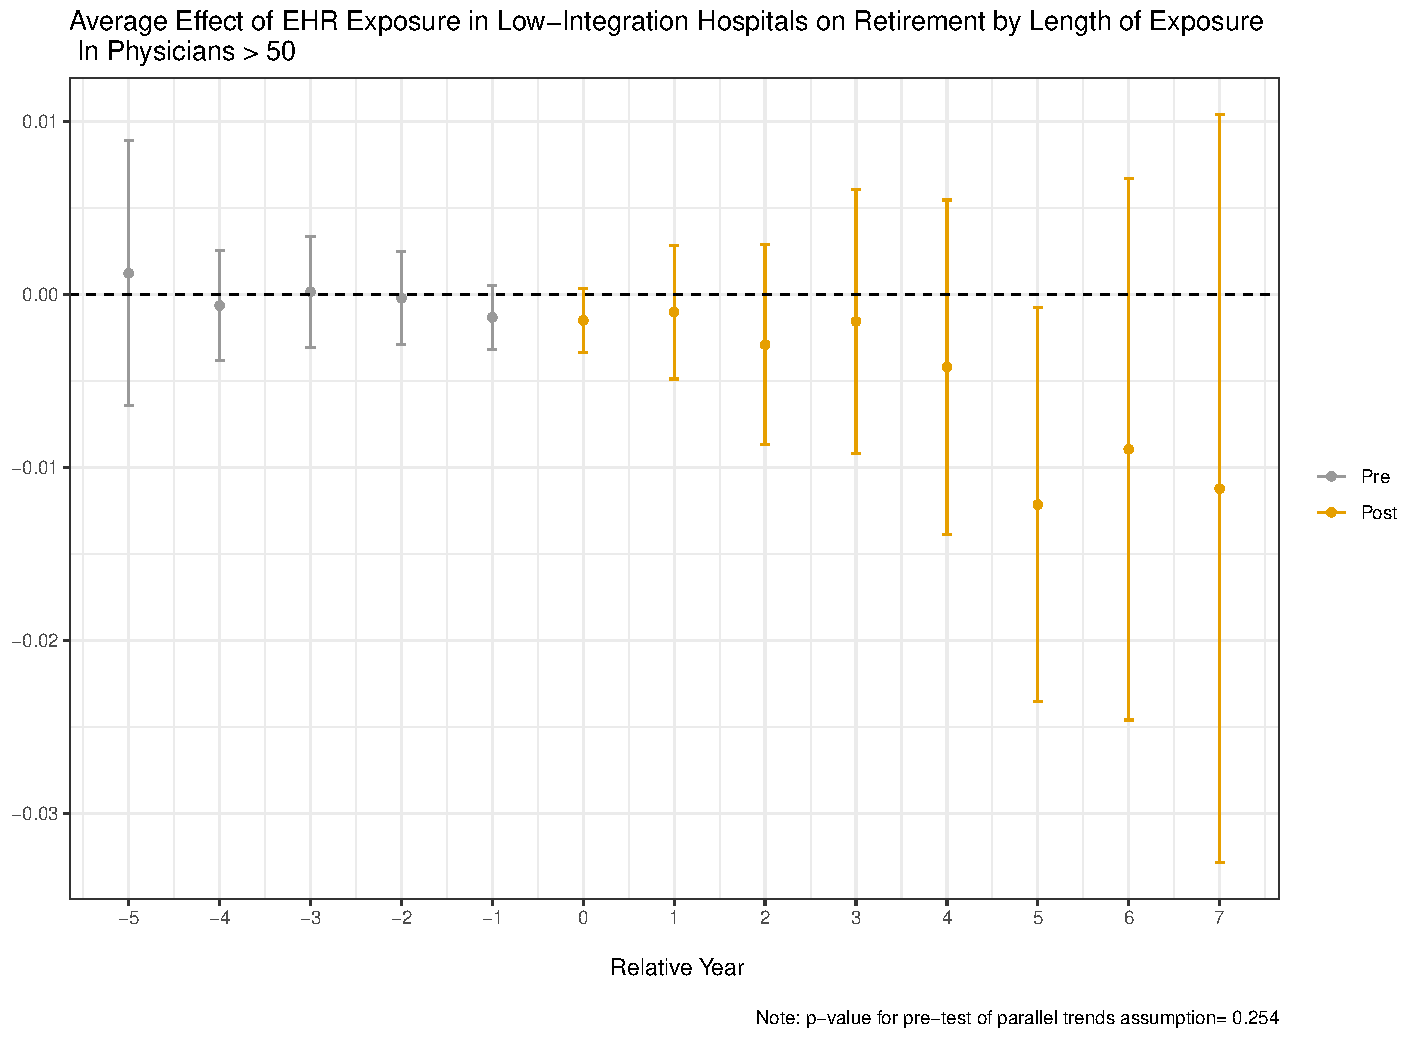
\includegraphics[width=\textwidth]{Objects/ggdid_retire_allEHR_old_li.pdf}
        \end{minipage}
        \label{fig:retiresecond}
\end{figure}



\section{Work Setting}

\section{Physician Productivity}

An important aspect in the implementation of EHRs is whether or not they increase productivity in users. Productivity, in this case, has two key determinants: the choice of physicians to learn and utilize the technology, and the realized quality/innovation of electronic health records themselves. Regarding the first determinant, I will assume that when a physician continues to work in an electronic record utilizing-hospital, they utilize the electronic health record system fully. That is, there are no physicians who stay actively working in a hospital but choose not to partake in the electronic health record used by the hospital. To understand the second determinant, the value added of electronic health records themselves, the sample of physicians is limited to those who have patients in hospitals even after EHR exposure. 

It is reasonable to believe that physicians are fully utilizing the EHRs in the hospital they work in, since by 2015 electronic health records were widely implemented and considered unavoidable. An objection to this assumption may be that older physicians stay in a hospital, but the hospital hires a data assistant to do technology work for the physician. In this case, the productivity gain could be from having the data assistant instead of EHR use. I investigate this below.

\subsection{Data Assistants}

One concern with this measure of productivity is that an increase in the number of patients seen by a physician could be caused by an outside factor that is also correlated with EHR adoption in hospitals. A logical outside factor could be the existence of employees with the purpose of utilizing electronic health records on a physician's behalf. Employees of this type are assigned a medical tax ID when working in hospitals; they have the following titles: Coding Specialist (Hospital Based), Health Information Technologist and Registered Record Administrator. I will refer to any employee in these categories as a data assistant. 

Using NPPES data on all NPIs and their tax information, I analyze the existence of data assistants in hospitals. Figure \textcolor{red}{number} is a frequency plot of the year of activation for every tax code that falls in the categories listed above. The total number of these registered employees is 875. The first data assistants ever registered were in 2005, when electronic medical records were being implemented. From 2005 to 2013, more 15-60 more employees were registered each year. The graph is clearly skewed towards later years, where a significant increase in the number of new data assistants occured in 2014. If hiring data assistants were directly correlated with both EHR implementation and physician frustration, one would expect the increase to occur from 2011-2012, when a majority of physicians were first exposed to EHRs. 


\vspace{5mm}
\begin{figure}[ht]
\caption{Frequency of Data Assistant Enumeration by Year}

    \label{fig:dataassistant_histogram}
\end{figure}

The total number of registered data assistants may not equal the true number of people doing a data assistant job in hospitals. However, under the assumption that the number of registered data assistants is proportional to the number of actual data assistants, the claim of no correlation still holds. 


\subsection{Event Study and Results}

The analysis in this section focuses on the effects of hospital EHR implementation on physician productivity within hospitals, measured by the total number of Medicaid patients billed in hospitals in a given year. The estimating equation is given as follows: 

\begin{equation*}
    y_{it}=\alpha_i+\delta_t+q_{it}'\lambda+\sum_{k=-5}^5 \beta_kz_{i,t-k} + \varepsilon_{it},
\end{equation*}

where $y_{it}$ is the number of patients, $\alpha_i$ and $\delta_i$ are physician and time fixed effects, $q_{it}$ are hospital characteristics such as number of beds and days open during the year, $z_{i,t-k}$ is an indicator for whether the physician was exposed to an EHR in any hospital in time $t-k$, and $\epsilon_{it}$ is a random error term. 

The identifying assumption is that physicians are exposed endogenously to electronic health records. That is, hospital management decides and implements EHRs, and this decision is not correlated with physician productivity or labor market decisions. This is not unreasonable for large hospitals with ample resources and many physicians. However, a small hospital may give experienced physicians some level of voice in the decision to implement new technologies. Results under this assumption are shown below, and  \textcolor{red}{the strength of this assumption is considered in the next section. } 

An event study plot containing estimates and confidence intervals of  $\{\beta_k\}_{k=-5}^5$  is given in in Figure \textcolor{red}{number}. The left hand side is the full sample of physicians at any experience level. As is standard in event studies, the identification of the coefficients depends on the assumption that there are no pre-trends. The p-value of a Wald test for pre-trends in both event studies indicate no observable pre-trends in the data.

For physicians at any experience level, EHR exposure yields no immediate affect on physician productivity, but leads to a clear increase in the number of patients seen beginning 2 years after exposure. After 5 years of exposure, physicians are seeing, on average, 93.67 more Medicaid patients per year. Relative to the mean in the year before exposure, 796.95, this is an 11.75\% increase in the number of patients seen. When the sample of physicians is limited to senior physicians (at least 35 years of experience), this effect disappears. In fact, the results show a slight decrease of \textcolor{red}{put the exact number here} in the number of patients seen in the year after exposure, and no effect following that year. This graph limits event time from -4 to 4 due to restricted sample size in year 2010 and 2014. 


\begin{figure}[ht]
\caption{}
        \begin{minipage}[b]{0.47\linewidth}
            \centering
            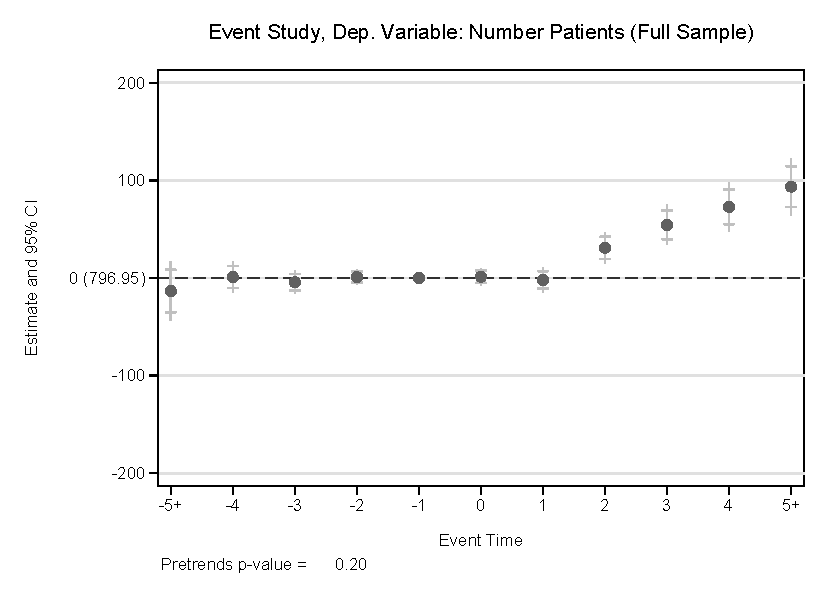
\includegraphics[width=\textwidth]{Objects/prod_eventstudy_fullsample.pdf}
        \end{minipage}
        \hspace{0.2cm}
        \begin{minipage}[b]{0.47\linewidth}
            \centering
            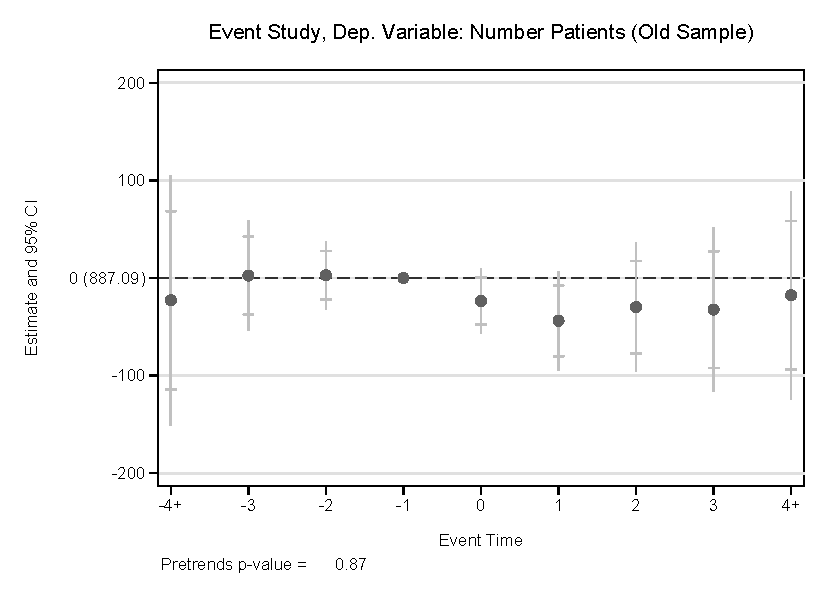
\includegraphics[width=\textwidth]{Objects/prod_eventstudy_oldsample.pdf}
        \end{minipage}
\end{figure}

\subsection{Relaxing Exogeneity of Implementation}


\textcolor{red}{I need to put somewhere that i dropped 2015 for this analysis since it cut off at a different point than the other years}

\renewcommand*{\bibfont}{\footnotesize}

\printbibliography

\newpage

\appendix

\section{}








\end{document}